\documentclass[../main.tex]{subfiles}

\begin{document}

\section{Prueba con solo la posición de las partículas. No la distancia.}

Sin las distancias es bastante rápido.
Lo que más tarda es la función computeDensity.

Ayer tuve que esperar, aproximadamente 3 hrs para 10 experimentos.
Eliminando el análisis con las distancias tuve que esperar medio minuto.

\subsection{Resultados}

Pues en la siguiente gráfica se observa la gran diferencia cuando solo se usa la posición de las partículas y no se usa la distancia entre las partículas.


\begin{figure}[ht!]
    \centering
    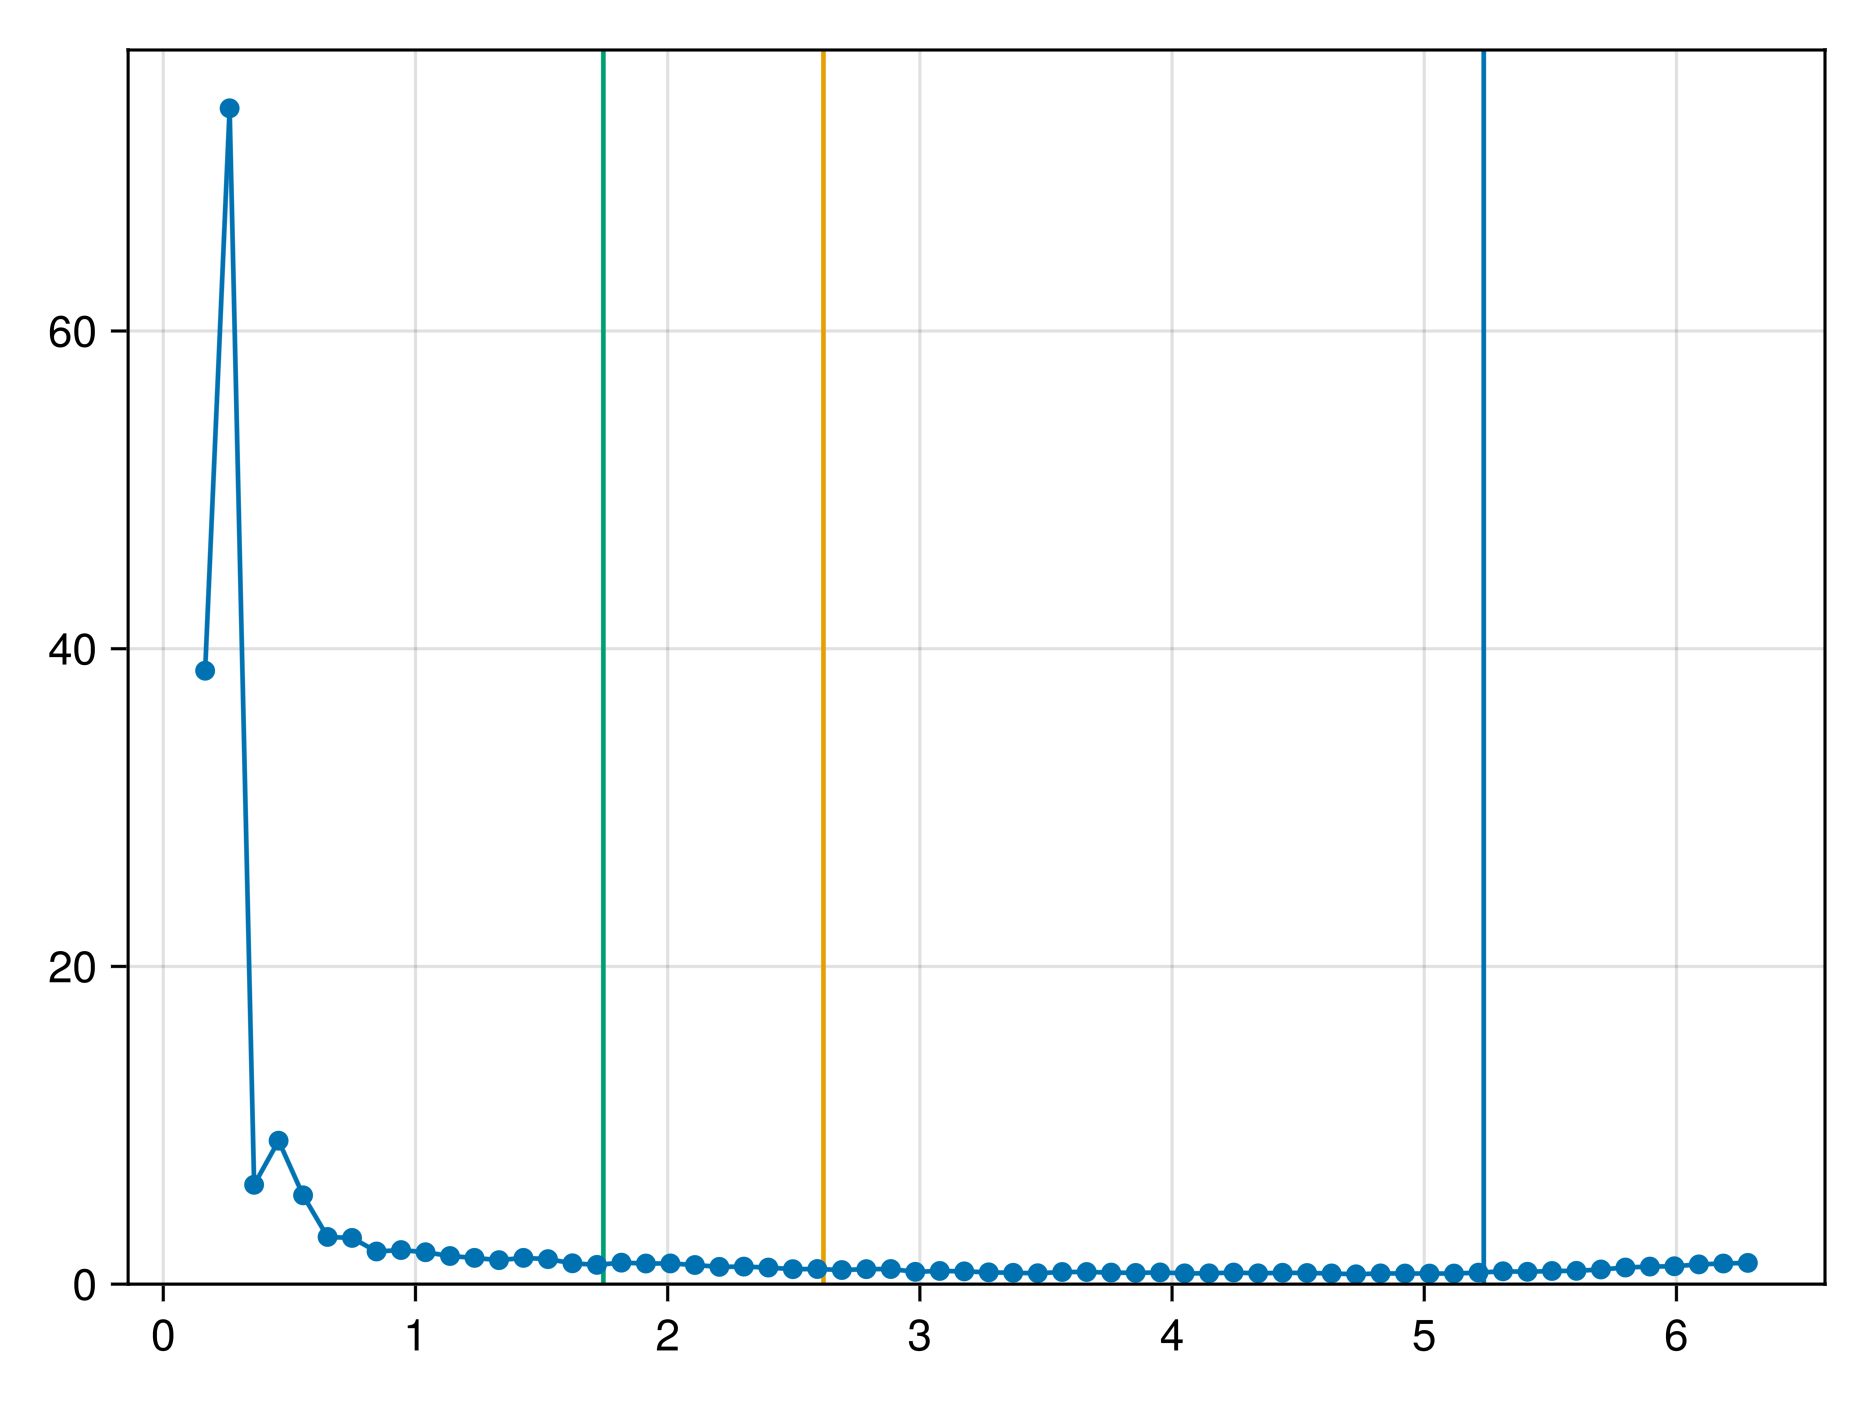
\includegraphics[width=0.9\textwidth]{../Figures/may6/fig_SqCorreccion_phi5_r.png}
    \caption{Factor de estructura con la corrección. \(\phi=5\%\). Las líneas verticales están ubicadas en \(|\vec{q}|=2\pi/1.2,~|\vec{q}|=2\pi/(2\cdot1.2),~|\vec{q}|=2\pi/(3\cdot1.2)\)}
\end{figure}


\begin{figure}[ht!]
    \centering
    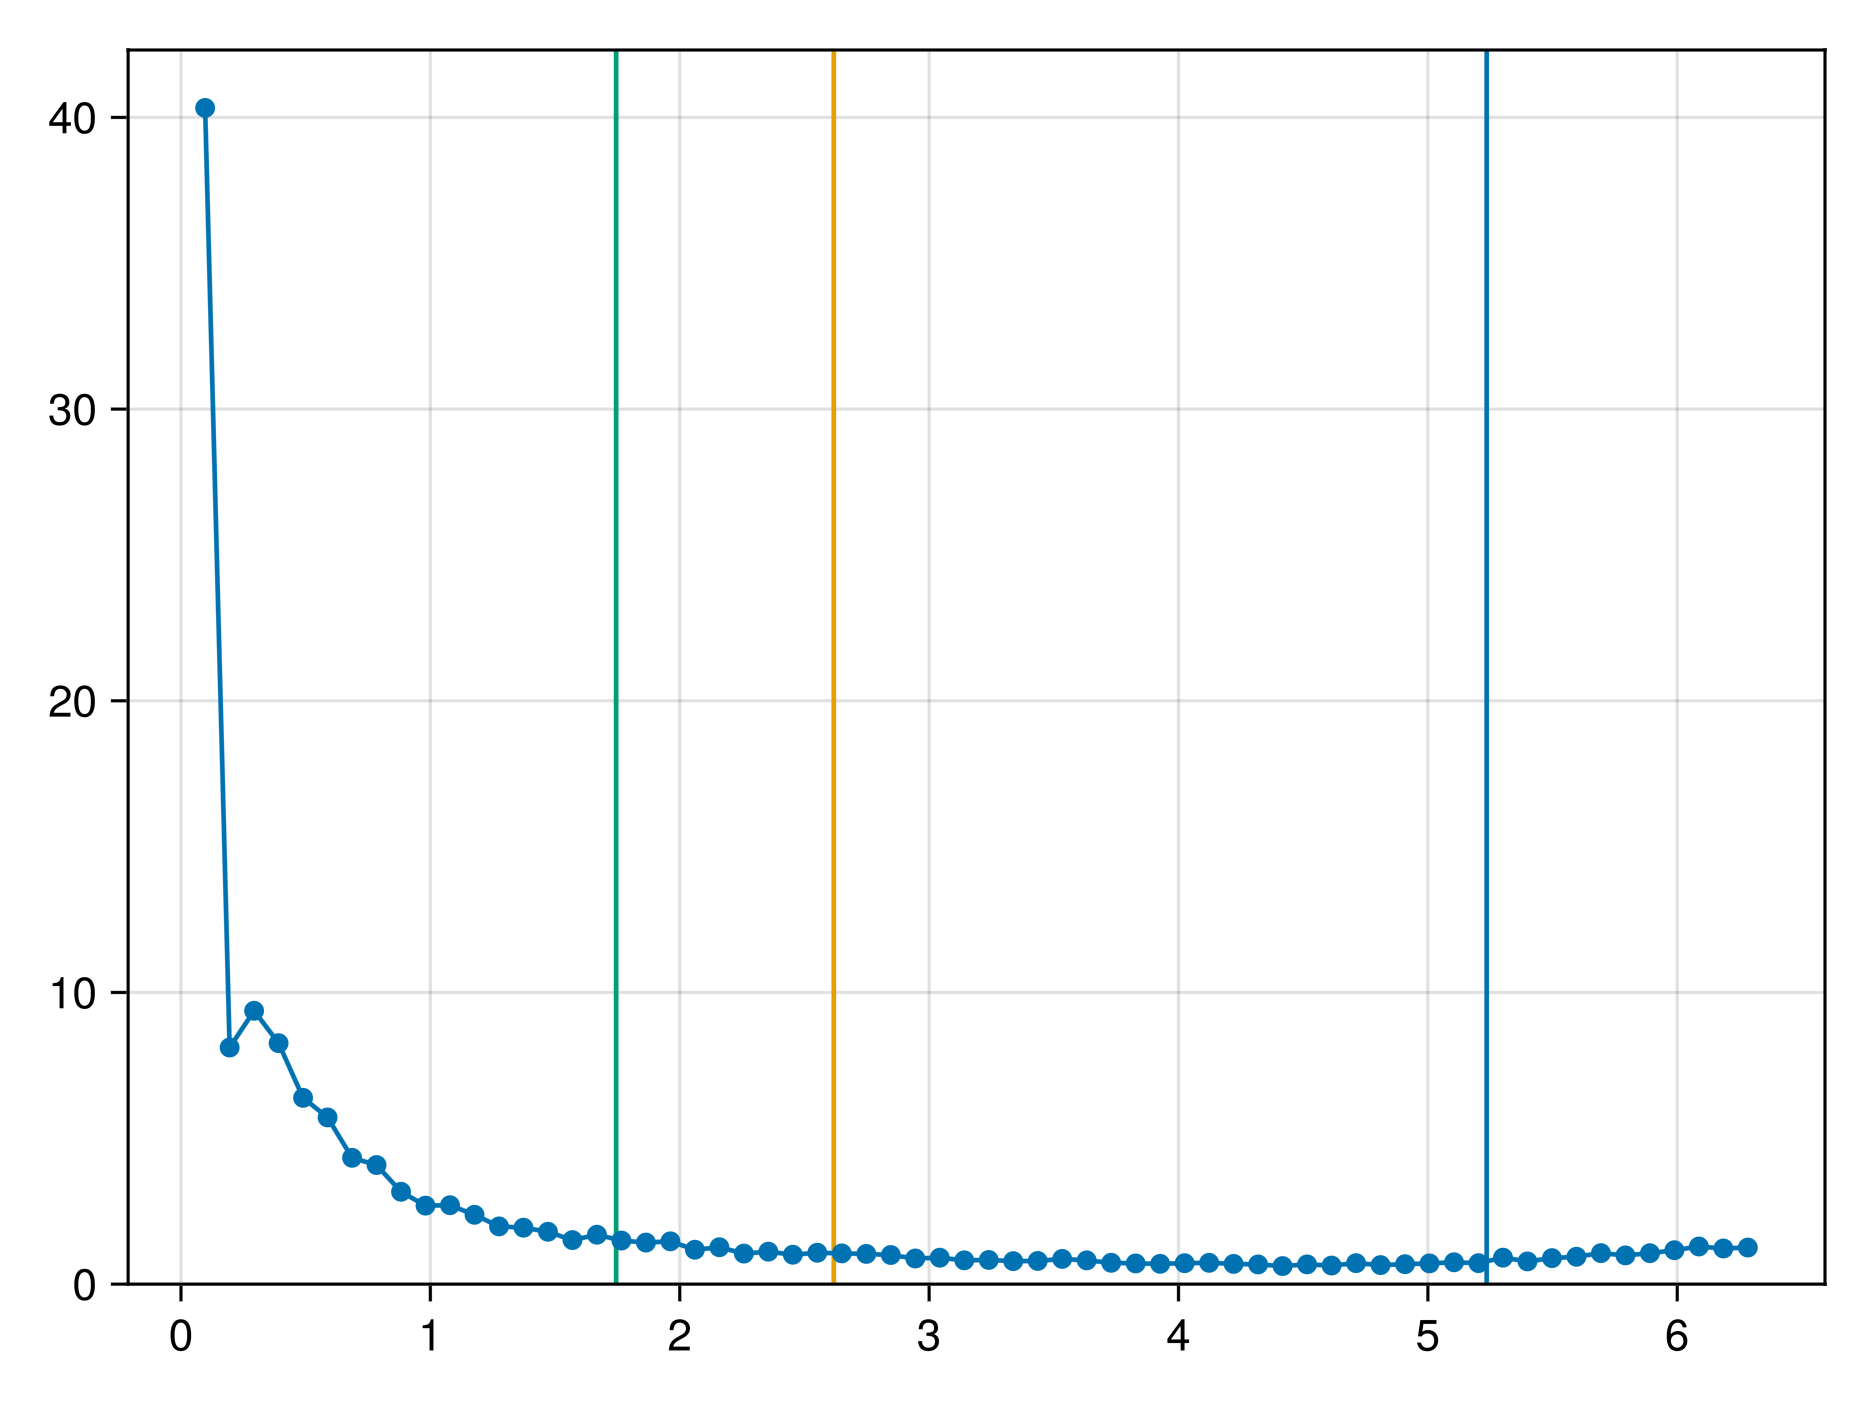
\includegraphics[width=0.9\textwidth]{../Figures/may6/fig_SqCorreccion_phi1_r.png}
    \caption{Factor de estructura con la corrección. \(\phi=1\%\). Las líneas verticales están ubicadas en \(|\vec{q}|=2\pi/1.2,~|\vec{q}|=2\pi/(2\cdot1.2),~|\vec{q}|=2\pi/(3\cdot1.2)\)}
\end{figure}

Pues si dan dos factores de estructura distintos, lo cuál es bueno saberlo.
Pero aún no se cómo interpretar estos análisis por lo que, por el momento, es \emph{información inútil} para mi.

\subsection{Comparación en \(t=0\) con timepo final usando distancias ente partículas}

8:43 se empezó a ejecutar el código.
A las 11:40 acabó.

\begin{figure}[ht!]
    \centering
    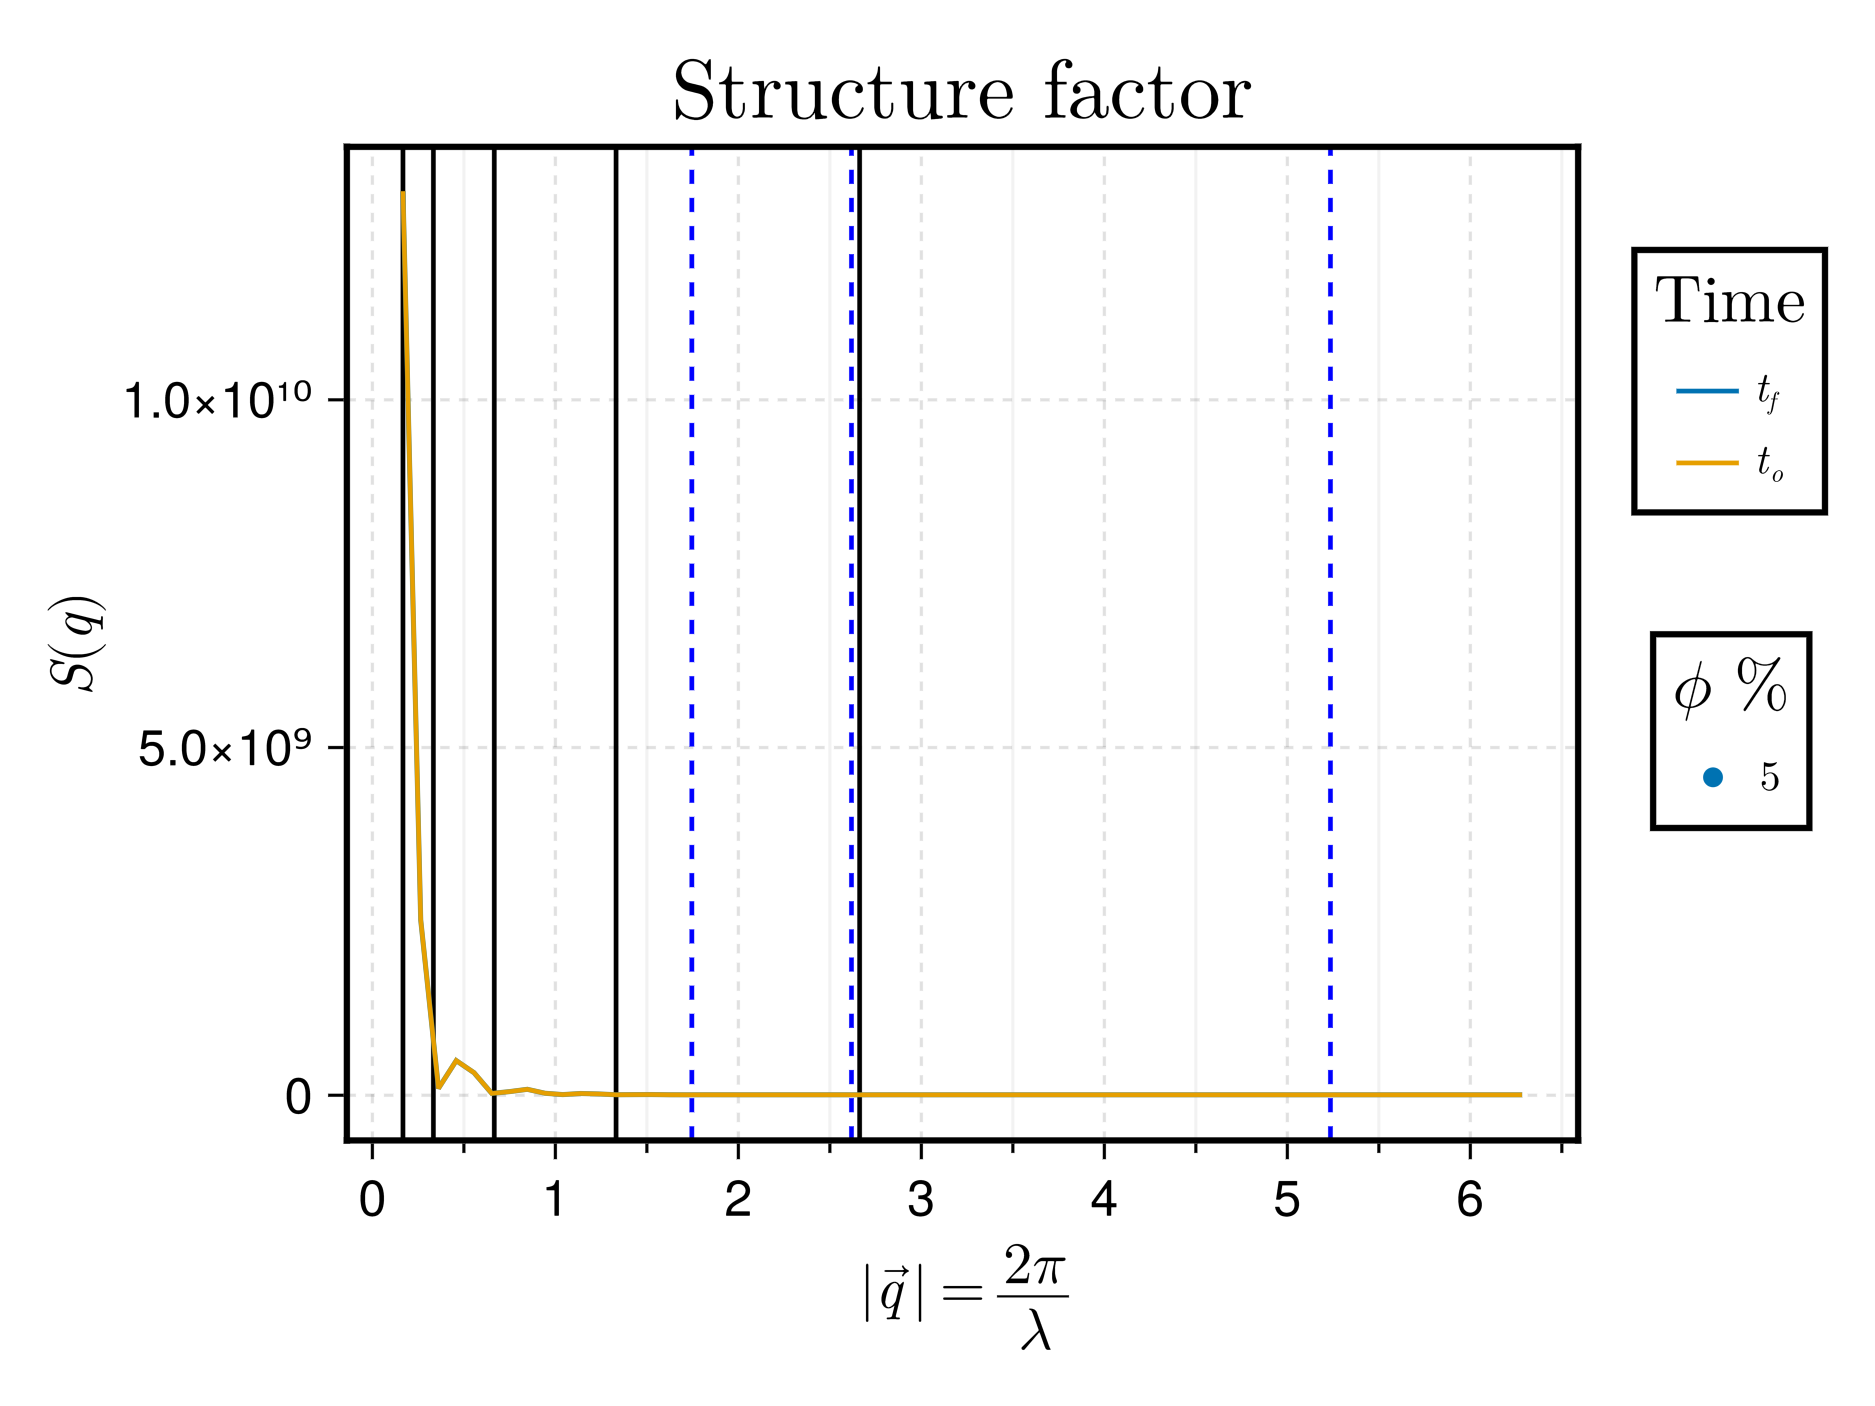
\includegraphics[width=0.9\textwidth]{../Figures/may6/fig_SqCorreccion_phi5_d_compt.png}
    \caption{Factor de estructura con la corrección. \(\phi=5\%\). 
    Las líneas verticales punteadas en azúl están ubicadas en \(|\vec{q}|=2\pi/1.2,~|\vec{q}|=2\pi/(2\cdot1.2),~|\vec{q}|=2\pi/(3\cdot1.2)\).
    Las líneas verticales punteadas en negro están ubicadas en \(|\vec{q}|\in\{2\pi/L,2\pi/L/2,2\pi/L/4,2\pi/L/8,2\pi/L/16\}\).
}
\end{figure}

De la figura anterior se puede observar que los picos a esas intensidades corresponden a la longitud de la caja.
Después hay un pico entre \(2\pi/L/2 \leq|\vec{q}|\leq 2\pi/L/4\).
Después de \(|\vec{q}|>2\pi/L/4\) parece que ya no hay picos.
Por lo tanto se hace un \emph{zoom} al disminuir el rango en el eje $y$.


\begin{figure}[ht!]
    \centering
    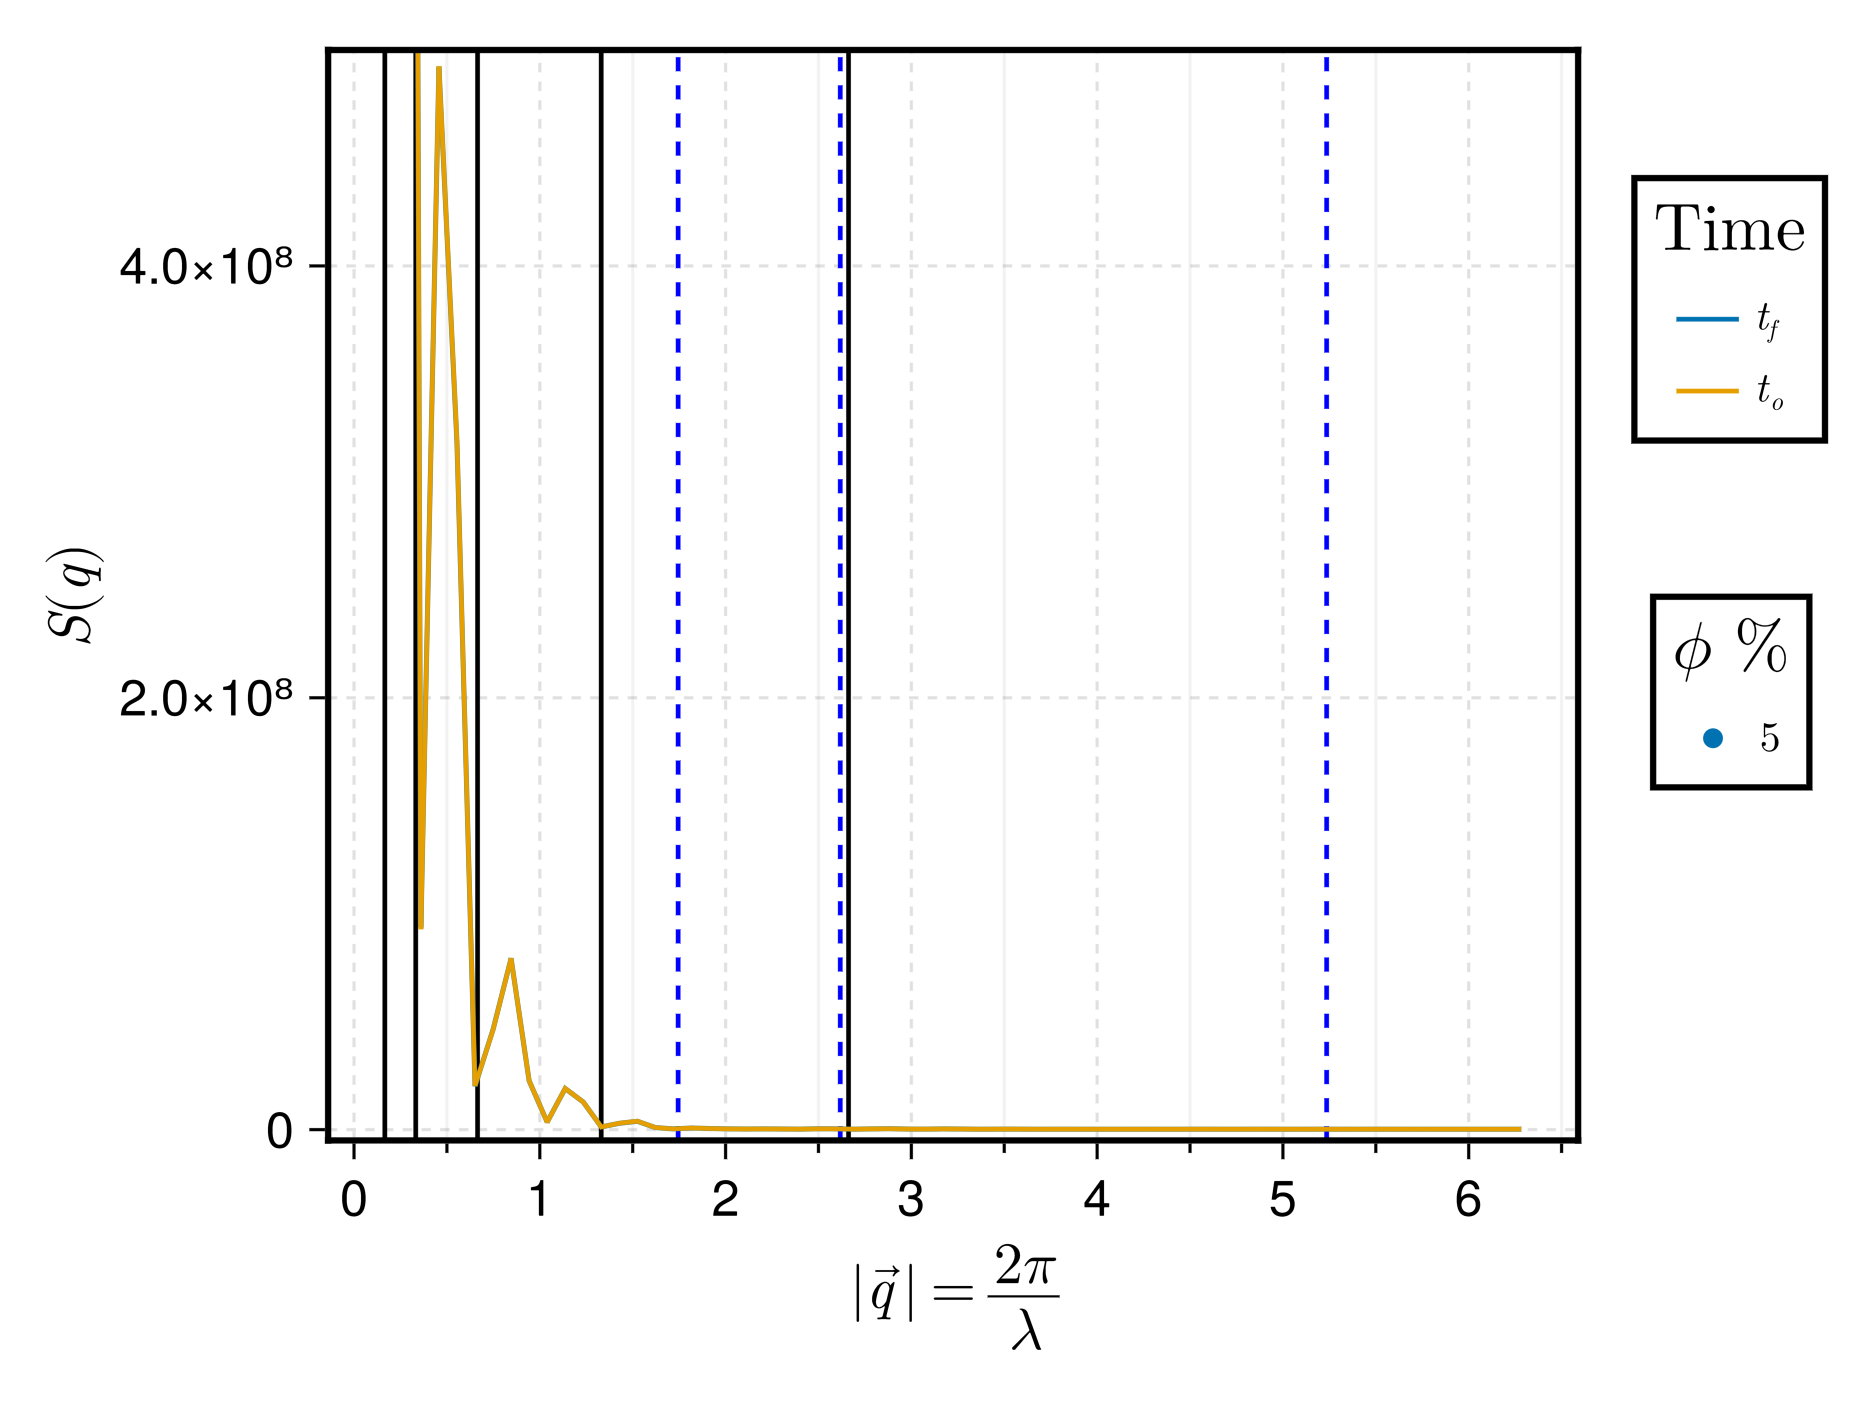
\includegraphics[width=0.9\textwidth]{../Figures/may6/fig_SqCorreccion_phi5_d_compt_zoom1.png}
    \caption{Factor de estructura con la corrección. \(\phi=5\%\). 
    Las líneas verticales punteadas en azúl están ubicadas en \(|\vec{q}|=2\pi/1.2,~|\vec{q}|=2\pi/(2\cdot1.2),~|\vec{q}|=2\pi/(3\cdot1.2)\).
    Las líneas verticales punteadas en negro están ubicadas en \(|\vec{q}|\in\{2\pi/L,2\pi/L/2,2\pi/L/4,2\pi/L/8,2\pi/L/16\}\).
}
\end{figure}

Este primer zoom ayuda a oberservar otros dos picos entre \(2\pi/L/4 \leq|\vec{q}|\leq 2\pi/L/8\).
Pero siguen sin apreciarse picos en términos de la longitud de enlace entre partículas patchy.
Por lo tanto se hace un segundo \emph{zoom}.


\begin{figure}[ht!]
    \centering
    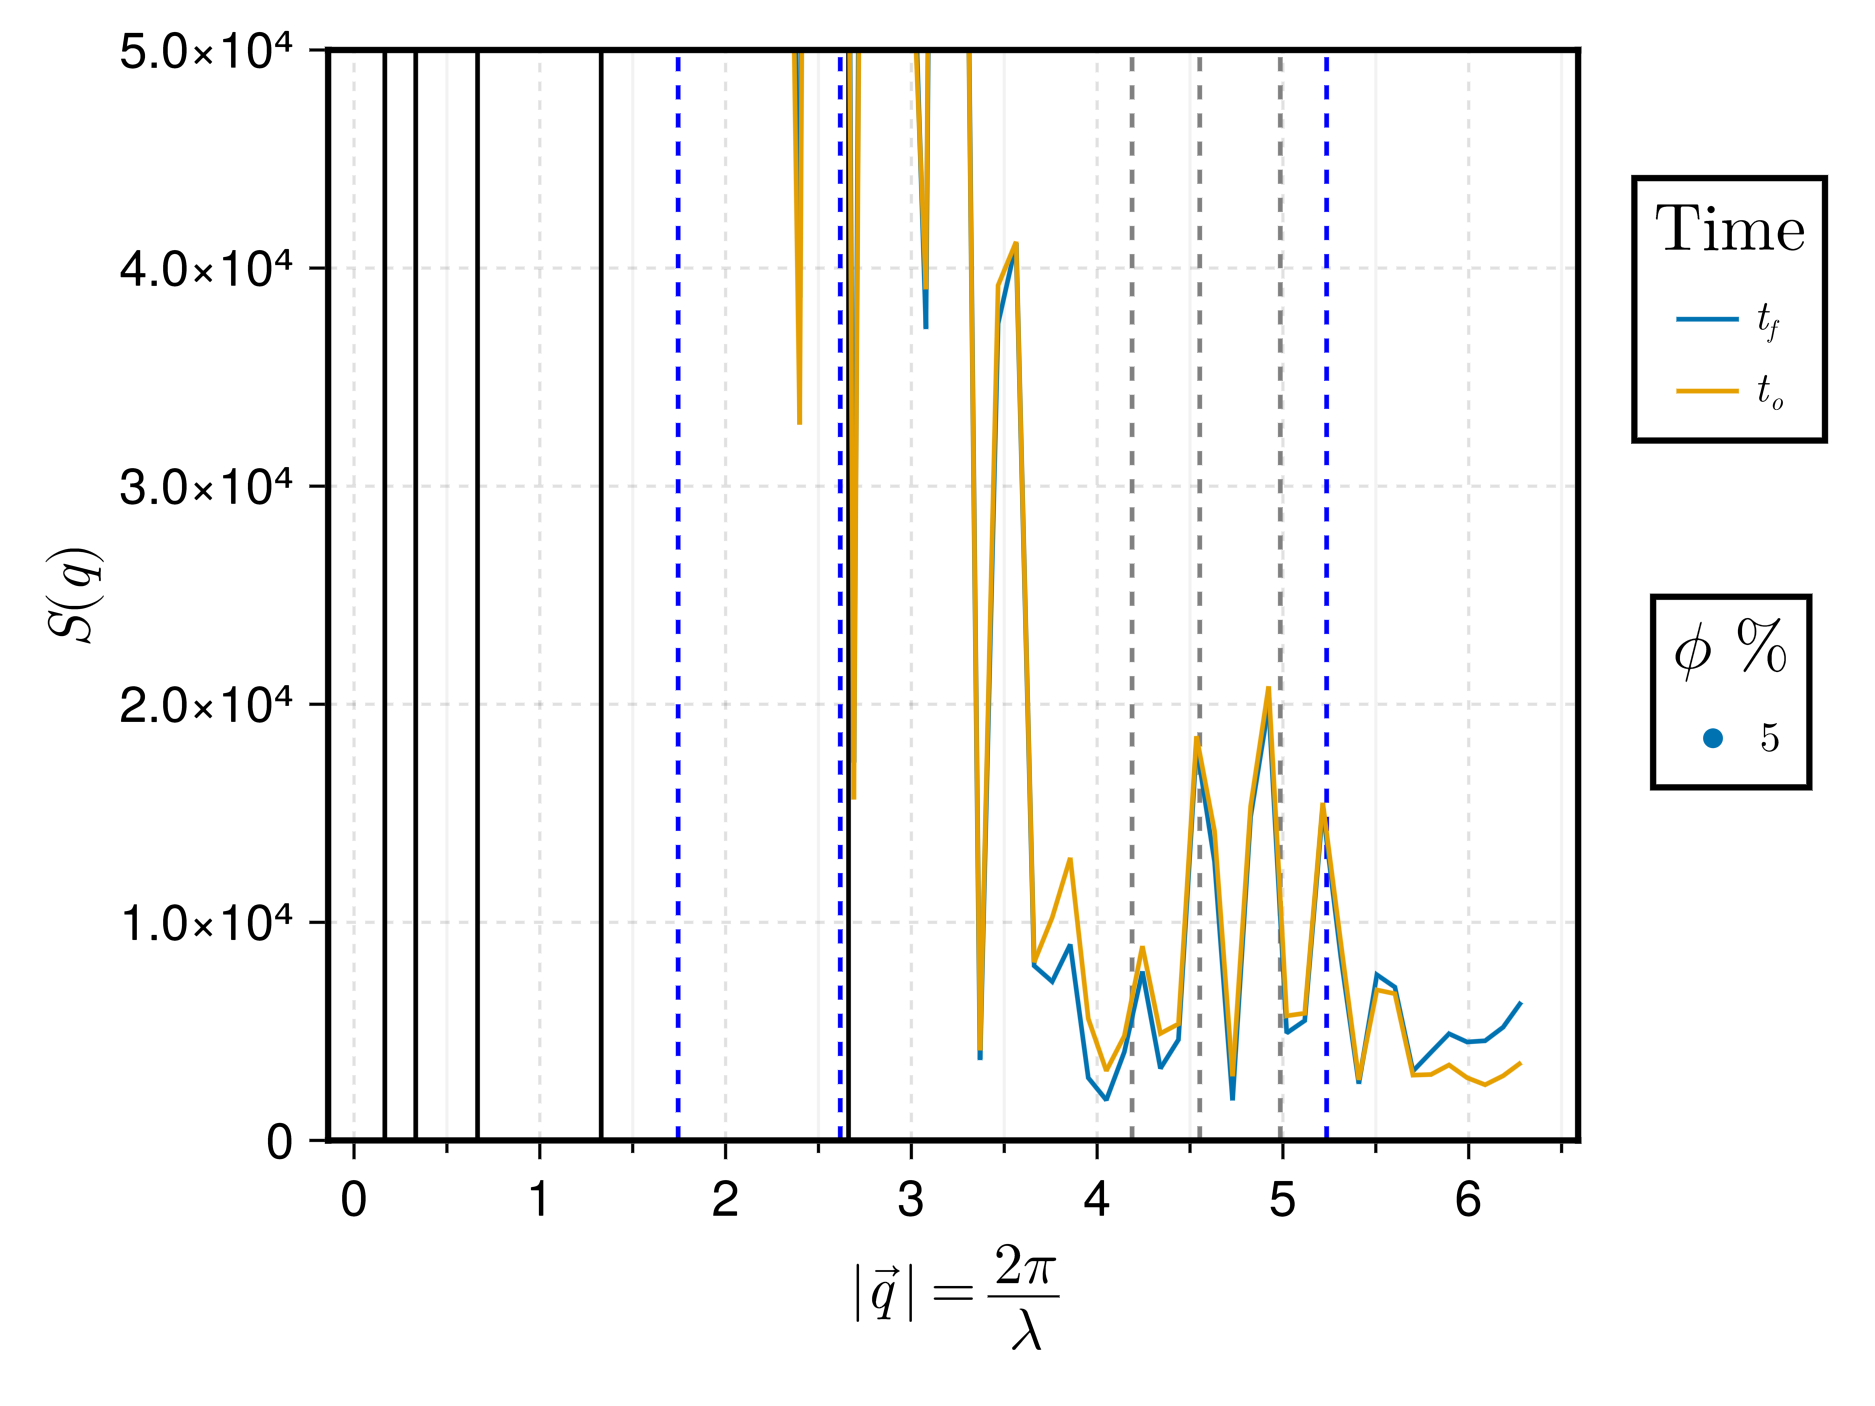
\includegraphics[width=0.9\textwidth]{../Figures/may6/fig_SqCorreccion_phi5_d_compt_zoom2.png}
    \caption{Factor de estructura con la corrección. \(\phi=5\%\). 
    Las líneas verticales punteadas en azúl están ubicadas en \(|\vec{q}|=2\pi/1.2,~|\vec{q}|=2\pi/(2\cdot1.2),~|\vec{q}|=2\pi/(3\cdot1.2)\).
    Las líneas verticales punteadas en negro están ubicadas en \(|\vec{q}|\in\{2\pi/L,2\pi/L/2,2\pi/L/4,2\pi/L/8,2\pi/L/16\}\).
}
\end{figure}

Finalmente observamos algunos picos en terminos de la longitud de enlace y una diferencia entre la configuración inicial y la configuración final.
Podemos observar que hay un pico exactamente en \(|\vec{q}|=2\pi/1.2\), la cuál es la distancia de enlace.
También se observan 3 picos siguientes marcados con una línea punteada gris en \(|\vec{q}|\in\{2\pi/(1.05\cdot1.2),2\pi/(1.15\cdot1.2),2\pi/(1.25\cdot1.2)\}\)

Por último, la \emph{gran} diferencia entre la primera configuración y la última configuración del sistema es magnitud del factor de estructura cuando \(\lambda\to1\).
Para la última configuración es considerablemente mayor que al inicio de la simulación.

%Considerando que la intensidad es debido a una interferencia constructiva 

\paragraph{Acerca de los picos de intensidad.}
Aún no me queda muy claro cómo surgen los picos.
Se menciona que tiene que ver con la interferencia cosntructiva y me ahce sentido, porque es una sumatoria de funciones trigonométricas, pero aún no me queda muy claro cómo se \emph{controla} la interferencia constructiva.
Está el producto punto y el cociente entre la longitud de onda con la distancia de las partículas.


Considerando que la mayor distancia que se puede encontrar entre partículas es \(L/2\) debido a las condiciones periódicas de frontera, podemos analizar facilmente le valor del factor de estructura para cuando \(\lambda=L\).

\begin{gather*}
    A = \sum_{j=1}^{N}\sum_{k=1}^{N}\cos\qty(\vec{q}\cdot\qty(\vec{r}_{j}-\vec{r}_{k})),\quad
    B = \sum_{j=1}^{N}\sum_{k=1}^{N}\sin\qty(\vec{q}\cdot\qty(\vec{r}_{j}-\vec{r}_{k})).
\end{gather*}

\dots 

\section{Discusión con Claudia acerca del factor de estructura}

Pues la intución está en que cometí un error en la forma en cómo se mapea el vector de onda \(\vec{q}\).
Caludia comentó que genera el vector de onda al definir un dominio para cada una de las componentes con un resolución mínima. 
Después agrupa los componentes en términos de magnitud.

Esa metodología difiere en cómo yo estoy realizando la binarización del vector de onda.
Porque yo divido entre magnitud y direcciones, por lo que no estoy realizando un muestreo adecuado en el espacio recíproco.

\subsection{Definición del espacio recíproco}

La forma en cómo lo sugiere Claudia es que se defina un máximo y un mínimo.
En este caso se tiene que \(\lambda\in\qty[1,L]\).
Pero esa restricción solamente afecta a la magnitud del vector de onda, no en las direcciones.
Por lo que es posible definir que las componentes del vector de onda tengan el siguiente dominio \(q_{i}\in\qty[-L,L]\), con \(i\) representando las direcciones cartesianas.

\paragraph{Implementación.}
Lo que cambie fue que ya no se generan puntos aleatorios, si no que se genera el vector unitario equiespaciado en coordenadas esféricas.
Después analice bien cómo estaba calaculando el producto punto y esta mal paralelizado/optimizado.

\subsection{Cálculo del producto punto optimizado}

La idea es realizar una multiplicación matricial para optimizar el cálculo del producto punto entre el vector de onda con el vector distancia.
Aprovecharé la propiedad conmutativa de la sumatoria para segmentar la sumatoria en los términos $A$ y $B$.

El vector de onda se puede representar por un vector columna, \[\vec{q}^{(\lambda)}=\begin{bmatrix}q_x^{(\lambda)} \\ q_z^{(\lambda)} \\ q_z^{(\lambda)}\end{bmatrix}.\]
Cómo se tienen \(N_{d}=\num{12.5d6}\) distancias, podemos representar todas las direcciones de 3 columnas con \(N_{d}\) renglones,
\begin{gather*}
    M_{d^{(jk)}} = 
        \begin{bmatrix}
            d_{x}^{(jk)} & d_{y}^{(jk)} & d_{z}^{(jk)} \\
            d_{x}^{(jk)} & d_{y}^{(jk)} & d_{z}^{(jk)} \\
            \vdots & \vdots & \vdots \\
            d_{x}^{(jk)} & d_{y}^{(jk)} & d_{z}^{(jk)}
        \end{bmatrix}.
\end{gather*}
Por lo tanto, se puede paralelizar el cálculo del producto punto para \(N_{d}\) direcciones usando una multiplicación matricial.
\begin{gather*}
    \vec{q}^{(\lambda)}\cdot\vec{d}^{(jk)} = 
    \begin{bmatrix}
            d_{x}^{(jk)} & d_{y}^{(jk)} & d_{z}^{(jk)} \\
            d_{x}^{(jk)} & d_{y}^{(jk)} & d_{z}^{(jk)} \\
            \vdots & \vdots & \vdots \\
            d_{x}^{(jk)} & d_{y}^{(jk)} & d_{z}^{(jk)}
        \end{bmatrix}
        \begin{bmatrix}q_x^{(\lambda)} \\ q_z^{(\lambda)} \\ q_z^{(\lambda)}\end{bmatrix}
\end{gather*}

Si la memoria RAM no da para almacenar la matriz \(M_{d^{jk}}\) se puede seccionar por subsecciones de 3 columnas por $n_{d}$ renglones y calcular la multiplicación matricial.

Posteriormente se evaluan las funciones trigonométricas usando el vector resultante cómo argumento, se suman y se guarda el resultado.



\end{document}
